El plan estratégico de la Universidad de Talca, destaca el apoyo a todo tipo de actividades emprendidas por las distintas Organizaciones Estudiantiles reconocidas. Entre las actividades destacan: recepción de alumnos nuevos, celebración del día de la carrera, actividades culturales y deportivas, actividades sociales, entre otras~\cite{5}.

\begin{figure}[!h]
	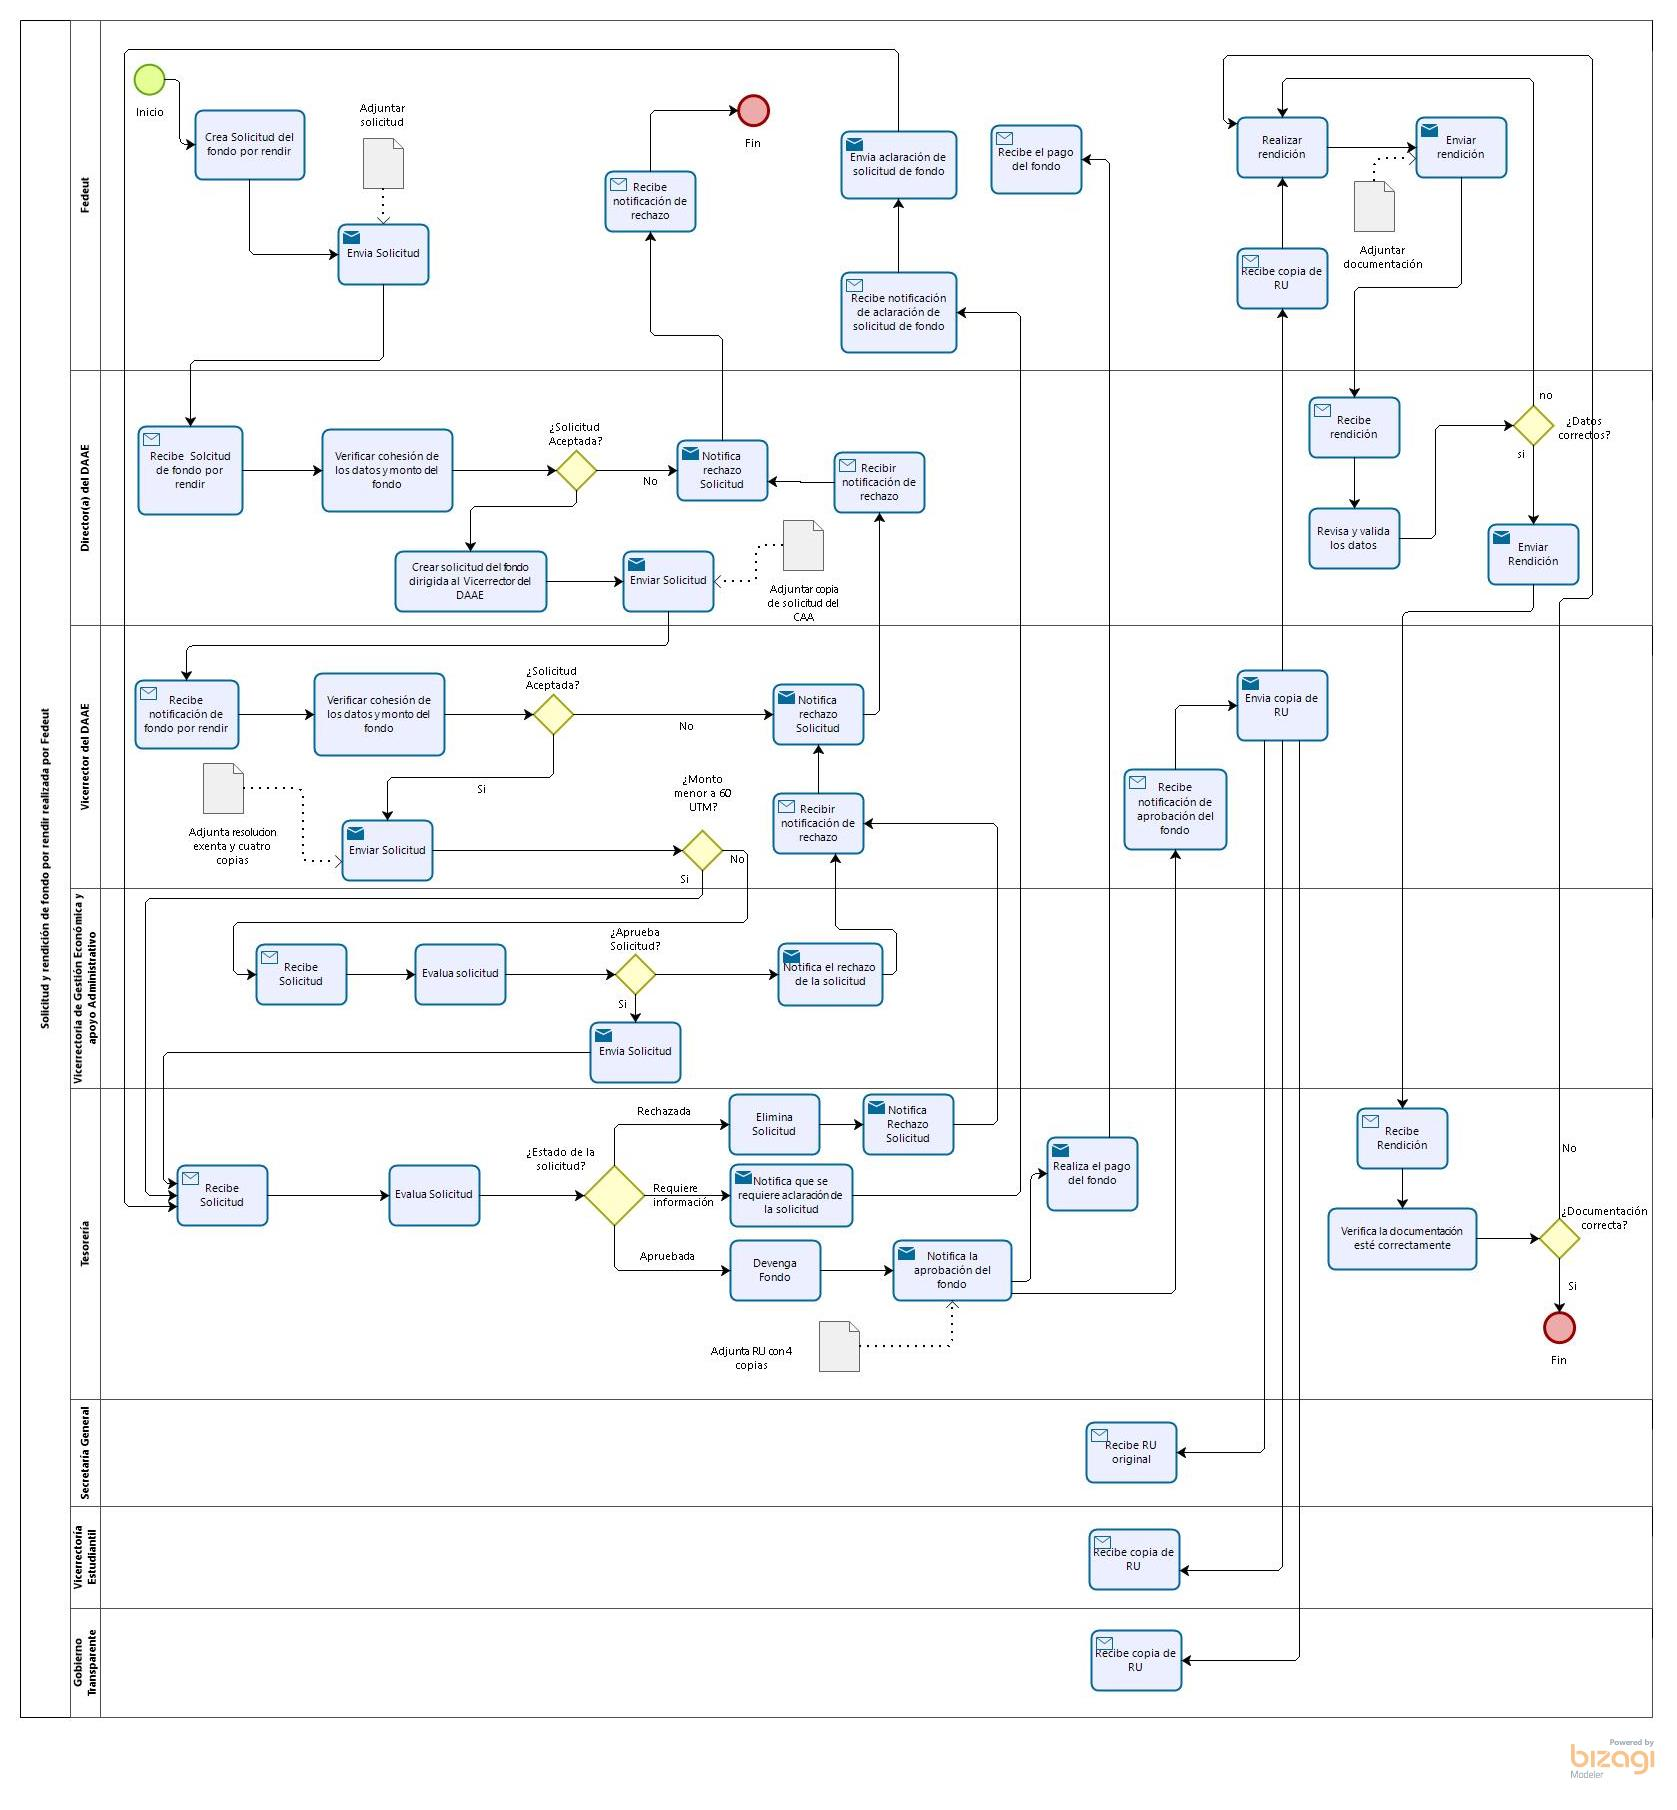
\includegraphics[width=\textwidth]{Imagenes/Solicitud_Federacion.jpg}
	\caption{\label{Solicitud_Federacion}Proceso fondos por rendir por parte de Fedeut.}
\end{figure}

Para la realización de estas actividades se debe seguir un procedimiento, el cual está estipulado en la RU N\grad 2083 creada el 12 de diciembre del 2017, la cual dice:

\begin{tasks}[counter-format = {tsk[A].}]
	\task \textbf{Caso Federación y Organizaciones Estudiantiles:}

	El Presidente, Tesorero o Secretario Financiero, es quien debe solicitar por escrito los Fondos aprobados para cada actividad al Director de DAAE, de la Vicerrectoría de Desarrollo Estudiantil, al menos 20 días previo al inicio de la actividad.

	El Director DAAE da visado a la solicitud de fondo para luego ser dirigida al Vicerrector de Desarrollo Estudiantil.

	El Vicerrector de Desarrollo Estudiantil luego de aprobar la solicitud de fondo, debe emitir una Resolución Exenta, original con cuatro copias y enviar a Contraloría de la Universidad de Talca para el respectivo control de legalidad. Una vez totalmente tramitado el acto administrativo, se distribuye de la forma siguiente: Original para el archivo de la Secretaría General, la primera copia  para el Departamento de Tesorería y Presupuesto, la segunda, copia para el archivo de la Vicerrectoría Estudiantil, la tercera, para la O.E. interesada y la cuarta para la unidad de Gobierno Transparente.

	Se puede apreciar con mayor detalle en la \textbf{Figura \ref{Solicitud_Federacion}}.

	\task \textbf{Caso de Centros de Alumnos}

	Se debe efectuar por escrito una solicitud de fondos al Director de Escuela respectivo, quién eleva la solicitud al Decano de la Facultad correspondiente o al Vicerrector de Desarrollo Estudiantil para el caso de las Escuelas no adscritas a una Facultad.

	El Decano o Vicerrector de Desarrollo Estudiantil procede a emitir una Resolución Exenta que transfiere los fondos para la actividad aprobada. Esta Resolución es emitida en original y cuatro copias, debiendo remitirse a controlaría universitaria para el respectivo control de legalidad.

	Una vez aprobada por Contraloría Interna y totalmente tramitada es enviada a Decano para su distribución de la siguiente forma: Original para Decanato, la primera copia para el Departamento de Tesorería y Presupuesto, la segunda copia para el archivo de la Facultad, la tercera copia es para la O.E. interesada y la cuarta a la Unidad de Gobierno Transparente.

	Se puede apreciar con mayor detalle en la \textbf{Figura \ref{Solicitud_CAA}}.
\end{tasks}

\begin{figure}[h!]
	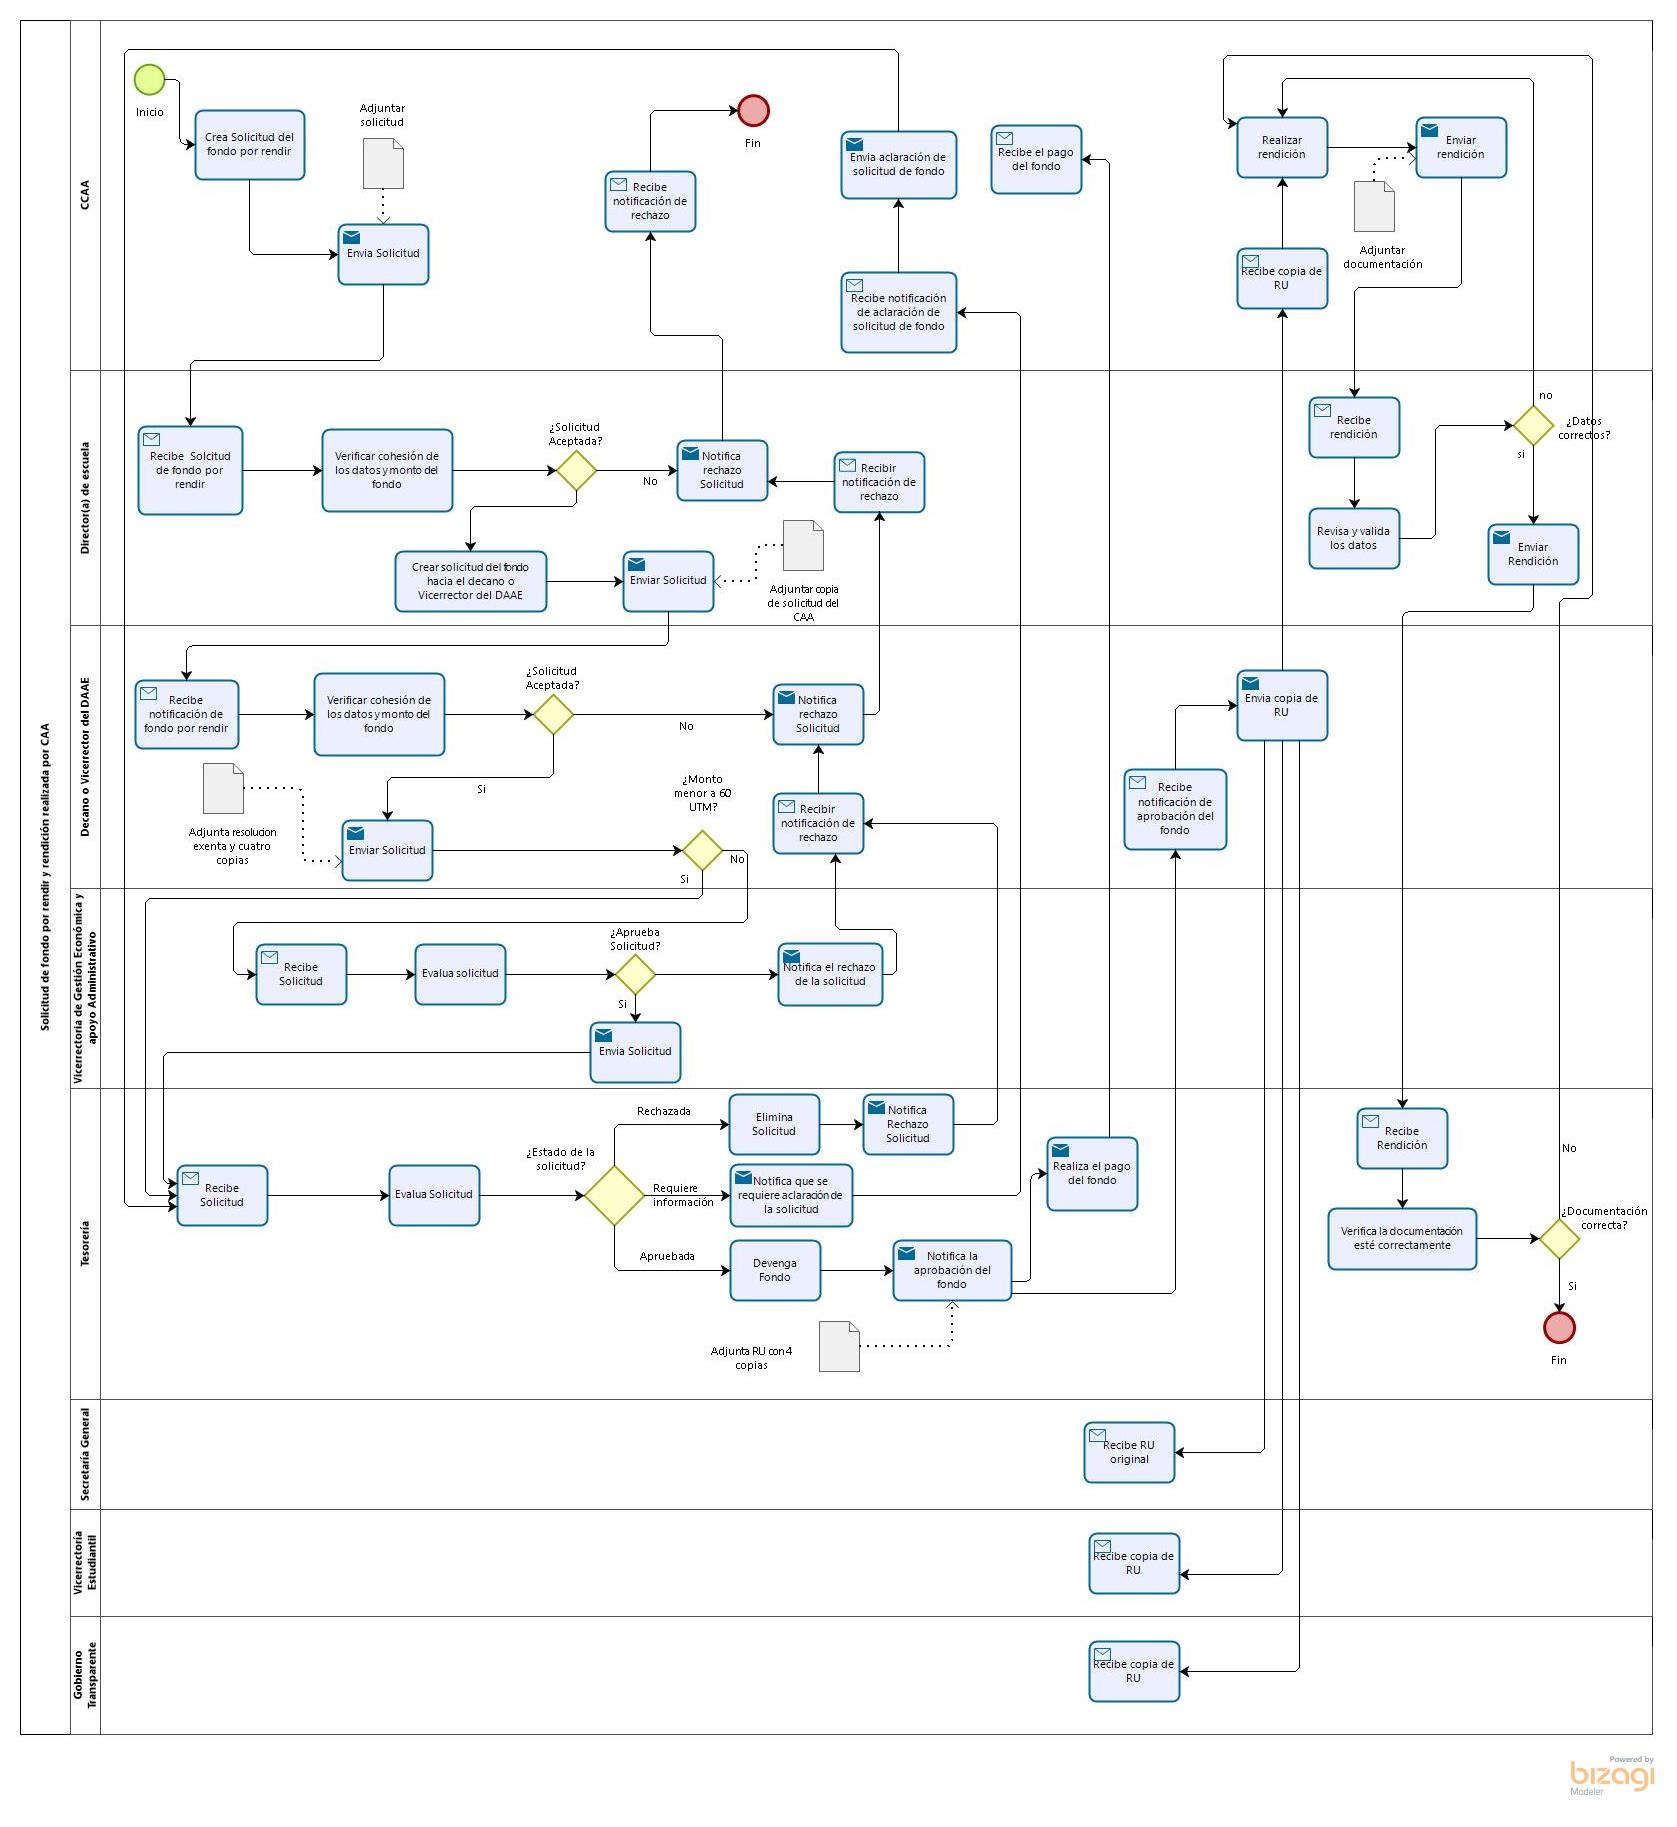
\includegraphics[width=\textwidth]{Imagenes/Solicitud_CCAA.jpg}
	\caption{\label{Solicitud_CAA}Proceso fondos por rendir por parte de CAA.}
\end{figure}

En ambos casos, el Departamento de Presupuesto hace responsable de la actividad presupuestaria correspondiente a la O.E que la solicita.

El Departamento de Tesorería emite el pago a nombre del Presidente o Tesorero o Secretario de Finanzas de la O.E. y adjunta la segunda copia de la Resolución al Comprobante de Egreso para la posterior rendición del Fondo.

Al representante de la O.E. se le asigna las siguientes responsabilidades:

\begin{itemize}
	\item Supervisar o realizar el cobro del documento de pago.
	\item Mantener un registro detallado de los gastos establecidos en el presupuesto de la actividad aprobada.
	\item Ejecutar/Realizar los gastos autorizados para la actividad.
	\item Rendir el Fondo asignado para la actividad.
	\item Respaldar gastos con la documentación idónea, tal como establece la Resolución Universitaria N\grad 522/1992, punto N\grad 12. 
\end{itemize} 

